\section{A Diversion Scenario: Highly Enriched Uranium}
\label{s_results}


% TODO: Actual #s: qty HEU, qty LEU, Power units, gaussian params etc.

% From google docs: CVT_research/collaborations/
\begin{figure}%[htbp!]
\begin{center}
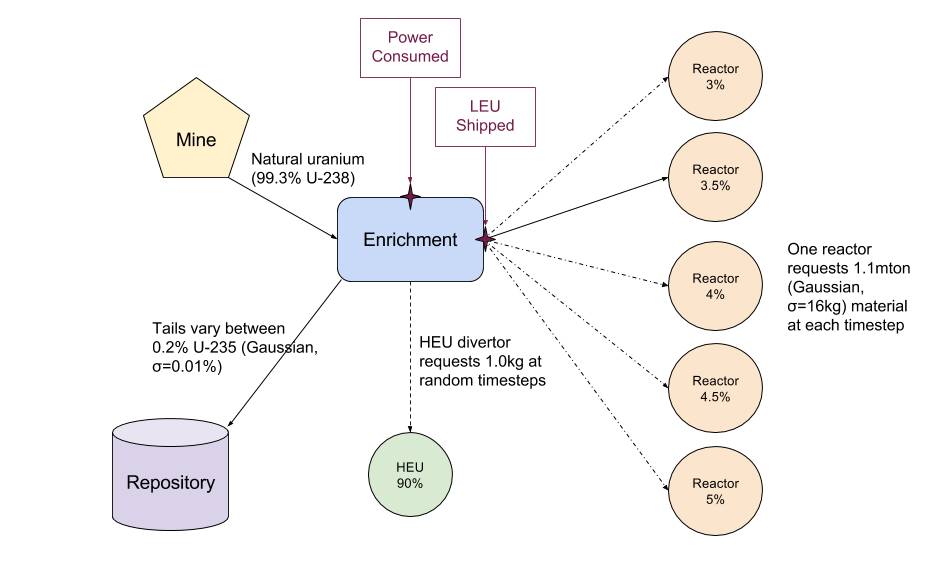
\includegraphics[natwidth=162bp,natheight=227bp, scale=0.4]{./figs/UM_multimodal_diagram.png}
\end{center}
\caption{Diversion scenario: Enrichment facility produced LEU for 5 different customers, as well as secretly making HEU occasionally.  Both LEU quantity and tails assays have slight variation to introduce ``noise'' into the system.}
\label{fig:scenario_layout}
\end{figure}


As a part of the \gls{CVT}\footnote{http://cvt.engin.umich.edu/}, \Cyclus is being used to generate multi-modal datasets with signatures of diversion with the goal of improving anomaly detection techniques. In the simplest implementation, \gls{HEU} is clandestinely produced and then diverted from an enrichment facility.  Figure \ref{fig:scenario_layout} illustrates a toy model of this portion of the fuel cycle. A facility such as a mine supplies natural uranium (0.7\% $^{235}$U) to an enrichment facility. The enrichment facility in turn receives requests for \gls{LEU} one of five enrichment levels (3-5\%) from several declared light-water reactors (ignoring the fuel fabrication facility for simplicity).  The enrichment facility also receives requests for 90\% enriched \gls{HEU} from an undeclared actor seeking to build a nuclear weapon. Material production for each facility is calculated once each month for a total of 200 months. At each timestep, the enrichment facility fulfills an order for one \gls{LEU} enrichment level, and sometimes produces small quantities of \gls{HEU} request. 

% ~/git/data_analysis/data/UM_data/multi_modal_v1.3/single_runs/INMM_051316
% Data from mm_5enrich_tinytails_insp.xml
\begin{figure}%
  \centering
    \begin{subfigure}{0.6\textwidth}
      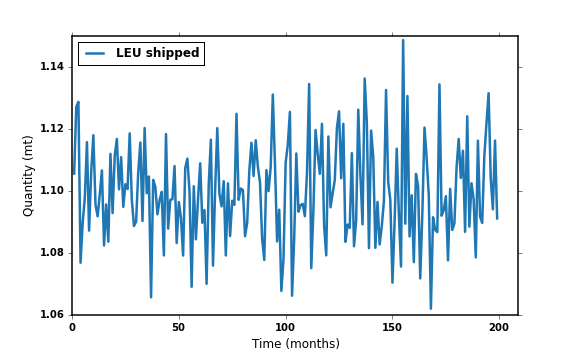
\includegraphics[natwidth=162bp,natheight=227bp, scale=0.6, clip=true]{./figs/mm_5enrich_tinytails_inspleu_shipped_E5.png}\\[-2ex]
            \label{fig:qty}
            \vspace*{-10mm}
    \end{subfigure}
    \begin{subfigure}{0.6\textwidth}
            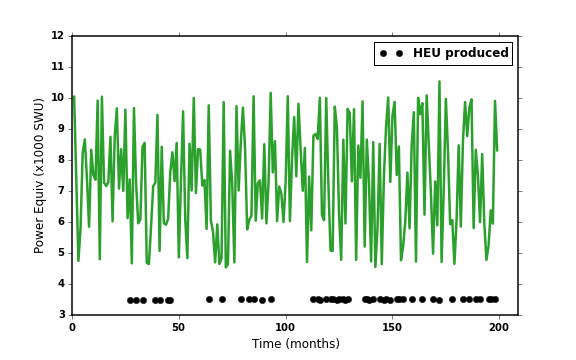
\includegraphics[natwidth=162bp,natheight=227bp, scale=0.6]{./figs/mm_5enrich_tinytails_inspEF_power_E5.png}
            \vspace*{-11mm}
            \label{fig:swu}
    \end{subfigure}
    \begin{subfigure}{0.6\textwidth}
            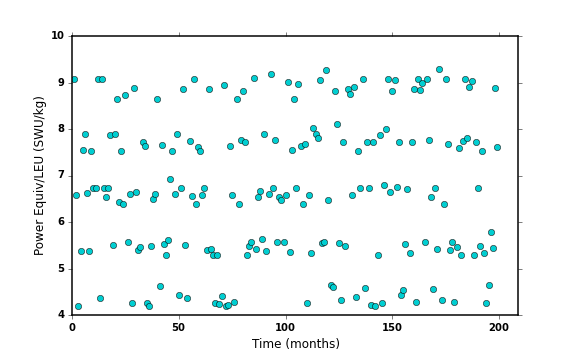
\includegraphics[natwidth=162bp,natheight=227bp, scale=0.6]{./figs/mm_5enrich_tinytails_inspratio_swu_leu.png}
            \label{fig:ratio}
    \end{subfigure}
    \caption{Time-series data for declared LEU production (top) and facility SWU consumption (middle). Green dots illustrate times at which HEU is also produced.  Theratio of power to LEU quantity (bottom) shows deviations from the mean when HEU is produced.}
    \label{fig:time_series}
\end{figure}


Figure \ref{fig:time_series} shows the time series data for declared production of \gls{LEU} (top) and the total \gls{SWU} consumed by the enrichment plant (middle) available to the inspector (\gls{SWU} can be used as a rough proxy for power consumption).  Months where \gls{HEU} is produced are denoted with green on the \gls{LEU} plot.  The \gls{HEU} signature is hidden in the material flow data because there is a gaussian variation in both the tails assay and the quantity of LEU produced.  Therefore it is not possible to detect diversion from the individual time-series data alone. However, the two signals can be combined to highlight the correlated signature of diverion. The bottom plot in Figure \ref{fig:time_series} shows time-series data for the ratio of SWU-consumption to declared \gls{LEU} production.  When the variation due to tails assay (``noise'') is sufficiently small, the deviations may be seen by eye. In practice, as the noise increases or the \gls{HEU} quantity reduces in amplitude, this signature quickly becomes difficult to detect by eye.

While this example is clearly a toy model, it illustrates the power of combining multiple signals from a scenario to improve detection capabilities. An important application of \Cyclus is to produce more complex synthetic datasets which are then provided to groups that specialize in developing advanced anomaly detection techniques. An ongoing collaboration with researchers at the Michigan Institute for Data Science\footnote{http://midas.umich.edu/} seeks to apply innovative anomaly detection techniques to these simulations to investigate detection limits for scenarios with sparse data sets or low signal-to-noise ratios.

